\documentclass[tikz]{standalone}
\usepackage{tikz}
\usepackage{amsfonts}
\usepackage{amssymb}
\begin{document}

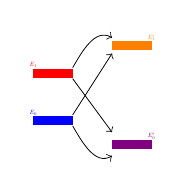
\begin{tikzpicture}
\coordinate (A) at (0.5,0.12);
\coordinate (B) at (1,0.5);
\coordinate (C) at (0.5,-0.62);
\coordinate (D) at (1,-1.0);
\coordinate (E) at (0.5,-0.48);
\coordinate (F) at (1,0.3);
\coordinate (A1) at (0.5,-0.02);
\coordinate (A2) at (1,-0.7);
\draw[red,fill=red] (0,0) -- (0.5,0) -- (0.5,0.1) -- (0,0.1) -- cycle;
\draw[blue,fill=blue] (0,-0.5)--(0.5,-0.5)--(0.5,-0.6)--(0,-0.6)--cycle;
\draw[->,line width=0.1 mm] (A) to[out=60,in=150] (B);
\draw[->,line width=0.1 mm] (C) to[out=-60,in=-150] (D);
\draw[->,line width=0.1 mm] (E) to (F);
\draw[->,line width=0.1 mm] (A1) to (A2);
\draw[orange,fill=orange] (1,0.35)--(1.5,0.35)--(1.5,0.45)--(1,0.45)--cycle;
\draw[violet,fill=violet] (1,-0.8)--(1.5,-0.8)--(1.5,-0.9)--(1.0,-0.9)--cycle;
\node[scale=0.22,red] at (0.0,0.15) {$E_1$};
\node[scale=0.22,blue] at (0,-0.45) {$E_0$};
\node[scale=0.22,orange] at (1.5,0.5) {$E_1 '$};
\node[scale=0.22,violet] at (1.5,-0.75) {$E_0 '$};
%\filldraw [draw=black] (A)  rectangle ++(B);
%\filldraw [draw=blue] (C)  rectangle ++(D);
\end{tikzpicture}

\end{document}